\subsection{Konstruktion des Modells}
\subsubsection{Allgemein}
Im Rahmen dieses Projektes wurden bereits umfangreiche Überlegungen angestellt, wie ein stabileres, leistungsstärkeres Modell unter Verwendung der größeren Motoren der Firma KEBA verwirklicht werden könnte.
Grundsätzlich basierten alle Überlegungen bezüglich der Konstruktion dieses Modells auf einer Fertigung aus Aluminium. Hierfür wurden im Projektverlauf die entsprechenden Aluminiumprofile beschafft, welche später beim Bau noch auf die optimale Länge zurecht geschnitten werden müssen. 
Im Zuge dieser Überlegungen wurde auch ein Aluminiumrohling in Form einer 16 mm Dicken Platte beschafft aus dem die Teile des Gelenks gefräst werden sollen.

\subsubsection{Gelenke}
Einen Knackpunkt bei der Konstruktion des Aluminiummodells stellte der Aufbau der einzelnen Gelenke dar. Die schlussendlich gewählte Herangehensweise wurde bereits in dieser Diplomarbeit im Kapitel "'Komponenten des Edubot Modells"' beschrieben. Grundgedanke der Gelenke ist die Erzeugung eines Bauteils der grob gesagt aussieht wie ein liegendes U. In den beiden Längsseiten des Us befinden sich Kugellager durch welche eine Verlängerung der Motorwelle führt. 
An diese Wellenverlängerung wird dann der eigentliche Arm befestigt. Durch diese Konstruktionsweise werden alle Kräfte die durch das Gewicht des Armes entstehen durch die Kugellager getragen und haben keinen Einfluss auf die Laufeigenschaften des Motors.
\newpage
\subsubsection{CNC Programmierung}
Die einzelnen Bauteile die zum Bau der im vorherigen Unterkapitel beschriebenen U-Förmigen Gelenke nötig sind wurden im Rahmen dieses Projektes als CNC Programm geschrieben und liegen dieser Arbeit bei. Als Werkzeug für die Erstellung der CNC Programme wurde die Software WinNC der Firma EMCO verwendet, welche in weiterer Folge auch für die Ausführung der Programme auf der schuleigenen Fräse verwendet werden kann. 
Grundsätzlich sind beim schreiben eines CNC Programmes nur die durch die Fräse auszuführenden Bewegungen und die jeweils benötigten Werkzeugoperationen aufzulisten. Für spezielle Operationen, wie beispielsweise das Fräsen einer Tasche oder das Bohren eines Gewindes stehen bereits vorgefertigte Operationen zur Verfügung die mit den richtigen Parametern aufgerufen werden müssen.
Leider gab es bei der Verwendung der WinNC Software Probleme mit der Lizenz, so dass zum Zeitpunkt der Anfertigung dieser schriftlichen Arbeit eine Simulation der CNC Programme nicht möglich war. Aus diesem Grund können hier keine Abbildungen gezeigt werden um die Einzelnen Bauteile zu präsentieren. Die Folgende Abbildung zeigt jedoch den einen Ausschnitt aus dem CNC Programm dass zur Erstellung eines Seitenteils des Gelenks verwendet werden kann, der gezeigte Ausschnitt dient dazu, Taschen für die Kugellager zu fräsen.

\begin{figure}[H]
\centering
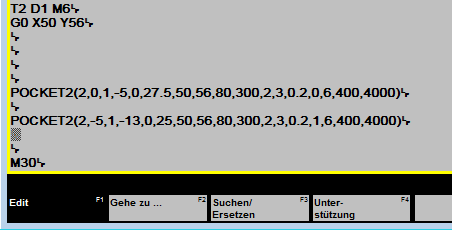
\includegraphics[width=9cm]{images/cncprogramm}
\caption{Screenshot eines CNC Programms in WinNC}
\end{figure}

\subsection{Sonstige Überlegungen}
Während der Planung der Mechanik des größeren Modells kamen wir unter Anderem zu dem Schluss, dass die Motoren nicht direkt mit den Armen verbunden werden sollten, sondern dass hier als Zwischenglied eine Übersetzung von Vorteil wäre. Diese Feststellung resultiert vor allem aus der Tatsache, dass die verwendeten Motoren sehr hohe Drehzahlen erreichen können und ihr maximaler Drehmoment im Gegenzug sehr begrenzt ist.
